\begin{figure}[H]
\noindent\begin{minipage}[t]{.49\textwidth}
% \begin{lstlisting}[language=Rust, label={lst:rustfivex}, caption={Rust code}, style=boxed, escapechar=`, basicstyle=\small]
\begin{lstlisting}[language=Rust, style=boxed, escapechar=`, basicstyle=\small]
fn rust_five_x(x: f32) -> f32 {`\label{line:rustfivex}`
  return 5.0*x;
}
extern "C" {
  fn c_five_x(x: f32) -> f32;
}
fn main() {`\label{line:fivexharness}`
  let x = 0.0.verifier_nondet();`\label{line:xcreate}`
  verifier_assume!(!isnan(x));`\label{line:xconstrain}`
  let c_res = unsafe {c_five_x(x)};`\label{line:fivexccall}`
  let rust_res = rust_five_x(x);`\label{line:fivexrustcall}`
  verifier_assert!(c_res==rust_res);`\label{line:fivexassert}`
}
\end{lstlisting}
\end{minipage}
%
\begin{minipage}[t]{.49\textwidth}
%\begin{lstlisting}[language=C, label={lst:cfivex}, caption={C code}, style=boxed, escapechar=`, basicstyle=\small]
\begin{lstlisting}[language=C, style=boxed, escapechar=`, basicstyle=\small]
float c_five_x(float x) {`\label{line:cfivex}`
  return x+x+x+x+x;
}
\end{lstlisting}
\end{minipage}
\caption{An example of a Rust program (left) that checks the equivalence of a native Rust-language function and an external C-language function (right).}
\label{fig:rustcfivex}
\end{figure}

%%%%%%%%%%%%%%%%%%%%%%%%%%%%%%%%%%%%%%%%%%%%%%%%%%%%%%%%%%%%%%%%%%%%%%%%%%%%%%%%%%%%%%%%%

\begin{figure}[H]
\noindent\begin{minipage}{.49\textwidth}
%\begin{lstlisting}[frame=tb, language=Rust, label={lst:rustsixx}, caption={Rust code.}, style=boxed, escapechar=`, basicstyle=\small]
\begin{lstlisting}[frame=tb, language=Rust, style=boxed, escapechar=`, basicstyle=\small]
fn rust_six_x(x: f32) -> f32 {`\label{line:rustsixx}`
  return 6.0*x;
}
\end{lstlisting}
\end{minipage}
%
\begin{minipage}{.49\textwidth}
%\begin{lstlisting}[frame=tb, language=C, label={lst:csixx}, caption={C Code.}, style=boxed, escapechar=`, basicstyle=\small]
\begin{lstlisting}[frame=tb, language=C, style=boxed, escapechar=`, basicstyle=\small]
float c_six_x(float x) {`\label{line:csixx}`
  return x+x+x+x+x+x;
}
\end{lstlisting}
\end{minipage}
\caption{An example of a program written in Rust (left) and a program written in C (right) which may seem to be equivalent.}
\label{fig:crustsixx}
\end{figure}

%%%%%%%%%%%%%%%%%%%%%%%%%%%%%%%%%%%%%%%%%%%%%%%%%%%%%%%%%%%%%%%%%%%%%%%%%%%%%%%%%%%%%%%%%

\begin{figure}[H]
\noindent\begin{minipage}{.47\textwidth}
%\begin{lstlisting}[language=C, label={lst:cstore}, caption={C equivalence.}, style=boxed, escapechar=`]
\begin{lstlisting}[language=C, style=boxed, escapechar=`]
float c_computation(float x) {
  float y = 2.0 * x;
  if(x < -1.0) {
    y += 1.0;
    verifier_equiv_store(y);
  }
  else if(x <= 0.0) {
    y -= 1.0;
    verifier_equiv_store(y);
  }
  else if(x <= 1.0) {
    y *= 2.0;
    verifier_equiv_store(y);
  }
  else {
    y /= 2.0;
    verifier_equiv_store(y);
  }
  return y;
}
\end{lstlisting}
\end{minipage}
%
\begin{minipage}{.52\textwidth}
\begin{lstlisting}[language=Rust, style=boxed, escapechar=`]
fn rust_computation(x: f32) -> f32 {
  let mut y = 2.0 * x;
  if x < -1.0 {
    y += 1.0;
    verifier_equiv_check(y);
  }
  else if x <= 0.0 {
    y -= 1.0;
    verifier_equiv_check(y);
  }
  else if x <= 1.0 {
    y *= 2.0;
    verifier_equiv_check(y);
  }
  else {
    y /= 2.0;
    verifier_equiv_check(y);
  }
  return y;
}
\end{lstlisting}
\end{minipage}
\caption{A demonstration of how the equivalence checking extensions to SMACK are used to verify equivalence of these C-language and Rust-language programs (left and right, respectively).}
\label{fig:storeequiv}
\end{figure}

%%%%%%%%%%%%%%%%%%%%%%%%%%%%%%%%%%%%%%%%%%%%%%%%%%%%%%%%%%%%%%%%%%%%%%%%%%%%%%%%%%%%%%%%%

\begin{figure}[H]
  \centering
  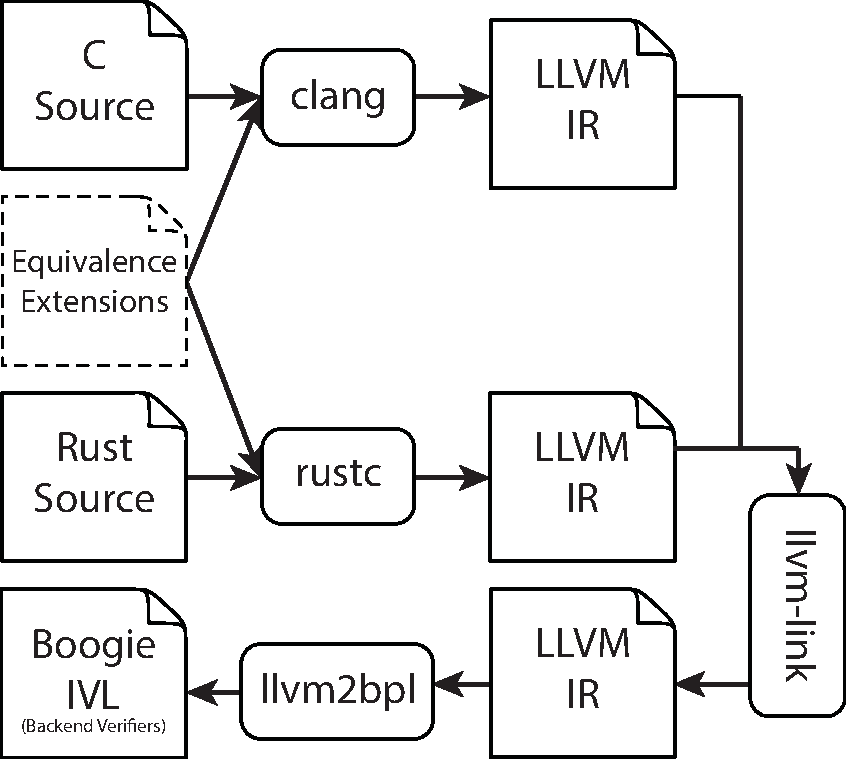
\includegraphics[width=0.92\textwidth]{chap4/fig/SmackEquiv.pdf}
  \caption{Equivalence checking extensions within SMACK.}
  \label{fig:toolflow}
\end{figure}

%%%%%%%%%%%%%%%%%%%%%%%%%%%%%%%%%%%%%%%%%%%%%%%%%%%%%%%%%%%%%%%%%%%%%%%%%%%%%%%%%%%%%%%%%

\begin{figure}[H]
\begin{minipage}[t]{.50\textwidth}
%\begin{lstlisting}[language=C, label={lst:nextafterc}, caption=nextafter in \texttt{musl}, style=boxed]
\begin{lstlisting}[language=C, style=boxed]
double nextafter(double x,
                 double y) {
    ...
    e = ux.i >> 52 & 0x7ff;
    verifier_store(e,``musl_e'');
    /* raise overflow if ux.f is
    infinite and x is finite */
    if (e == 0x7ff)
        FORCE_EVAL(x+x);
    ...
}
\end{lstlisting}
\end{minipage}
\begin{minipage}[t]{.50\textwidth}
%\begin{lstlisting}[language=Rust, label={lst:nextafterrs}, caption=nextafter in Rust, style=boxed]
\begin{lstlisting}[language=Rust, style=boxed]
fn nextafter(x:f64, y:f64) {
    ...
    let e=ux_i.
         wrapping_shr(52&0x7ff);
    verifier_comp(e,``musl_e'');
    // raise overflow if ux.f is
    // infinite and x is finite
    if e == 0x7ff {
        force_eval!(x + x);
    }
    ...
}
\end{lstlisting}
\end{minipage}
\caption{An example of how SMACK found a control-flow divergence in the implementations for the {\tt nextafter} functions as implemented in C (left) and Rust (right).}
\label{fig:nextaftercrs}
\end{figure}

%%%%%%%%%%%%%%%%%%%%%%%%%%%%%%%%%%%%%%%%%%%%%%%%%%%%%%%%%%%%%%%%%%%%%%%%%%%%%%%%%%%%%%%%%

\begin{table}[H]\centering
\caption{Rust and \texttt{musl} equivalence results.}\label{tab:rustmusl}
\vspace{1em}
\resizebox{\columnwidth}{!}{
\begin{tabular}{lrrrrrrrr}\toprule
Name &Status & Boogie/CVC5 &Boogie/Z3&Corral&Unroll &Inputs &SLoC \\\midrule
ceil & Equivalent & TO & 86.4$\pm$1.78s&TO &N/A &(f64) &88 \\
ceilf &Equivalent & TO &2.2$\pm$0.07s &2.6$\pm$0.03s &N/A &(f32) &76 \\
copysign &Equivalent & 5.4$\pm$0.51s &1.5$\pm$0.03s &3$\pm$0.06s &N/A &(f64, f64) &15 \\
copysignf &Equivalent & 2.4$\pm$0.26s &1.4$\pm$0.06s &2.2$\pm$0.06s &N/A &(f32, f32) &17 \\
fabs &Equivalent & 2.7$\pm$0.22s &1.9$\pm$0.05s &5.6$\pm$0.15s &N/A &(f64) &38 \\
fabsf &Equivalent & 2.0$\pm$0.19s &1.6$\pm$0.04s &2.5$\pm$0.09s &N/A &(f32) &38 \\
fdim &Equivalent & 5.8$\pm$0.18s &1.6$\pm$0.04s &9.2$\pm$0.06s &N/A &(f64, f64) &22 \\
fdimf &Equivalent & 5.0$\pm$0.18s&1.6$\pm$0.03s &3.1$\pm$0.07s &N/A &(f32, f32) &22 \\
floor &Equivalent & TO & 113.5$\pm$2.85s &TO &N/A &(f64) &87 \\
floorf &Equivalent &  TO &3.2$\pm$0.07s &3.5$\pm$0.12s &N/A &(f32) &77 \\
fmax &Equivalent & 4.7$\pm$0.22s &6.2$\pm$0.11s &52.4$\pm$2.69s &N/A &(f64, f64) &15 \\
fmaxf &Equivalent & 3.3$\pm$0.07s&2.8$\pm$0.11s &7.9$\pm$0.04s &N/A &(f32, f32) &15 \\
fmin &Equivalent & 4.9$\pm$0.12s &21.5$\pm$0.34s &110.7$\pm$2.96s &N/A &(f64, f64) &15 \\
fminf &Equivalent & 3.1$\pm$0.18s&7.4$\pm$0.15s &8.8$\pm$0.22s &N/A &(f32, f32) &15 \\
fmod &Equivalent & TO &22.9$\pm$0.64s &83$\pm$0.91s &2 &(f64, f64) &128 \\
fmodf &Equivalent & TO &183.4$\pm$3.5s &366.9$\pm$5.12s &2 &(f32, f32) &129 \\
frexp &Equivalent & TO & 22.8$\pm$0.85s &TO &3 &(f64, i32) &38 \\
frexpf &Equivalent & TO& 10.5$\pm$0.08s &TO &3 &(f32) &39 \\
ilogb &Equivalent & 3.0$\pm$0.16s &1.4$\pm$0.09s &2.5$\pm$0.06s &N/A &(f64) &52 \\
ilogbf &Equivalent & 2.9$\pm$0.17s &1.8$\pm$0.03s &3$\pm$0.1s &N/A &(f32) &52 \\
modf &Equivalent & TO & 53.2$\pm$0.92s &TO &N/A &(f64) &55 \\
modff &Equivalent & TO & 60.1$\pm$1.45s &TO &N/A &(f32) &56 \\
nextafter &Equivalent & TO &44.3$\pm$0.77s &12.3$\pm$0.41s &N/A &(f64, f64) &59 \\
nextafterf &Equivalent & TO &28.2$\pm$0.21s &11.1$\pm$0.37s &N/A &(f32, f32) &58 \\
remquo &Equivalent & TO & 210.8$\pm$4.25s &TO &1 &(f64, f64) &164 \\
remquof &Equivalent & TO & 363.3$\pm$10.35s &TO &2 &(f32, f32) &164 \\
rint &Equivalent & 7.5$\pm$0.40s &12.1$\pm$0.28s &50.8$\pm$0.69s &N/A &(f64) &68 \\
rintf &Equivalent & 3.1$\pm$0.15s &5.4$\pm$0.15s &9.9$\pm$0.16s &N/A &(f32) &70 \\
round & Equivalent & 434$\pm$14.47s&TO &TO &N/A &(f64) &55 \\
roundf &Equivalent & 61.6$\pm$2.3s &285$\pm$7.25s &237$\pm$6.84s &N/A &(f32) &58 \\
scalbn &Equivalent & 21.8$\pm$1.45s &207.8$\pm$3.6s &652$\pm$11.79s &N/A &(f64, i32) &58 \\
scalbnf &Equivalent & 8.2$\pm$0.225s &34.1$\pm$0.64s &62.3$\pm$1.91s &N/A &(f32, i32) &57 \\
trunc &Equivalent & 6.8$\pm$0.28s & 2.56$\pm$0.05s &TO &N/A &(f64) &50 \\
truncf &Equivalent & 2.1$\pm$0.11s&25.3$\pm$0.21s &15.1$\pm$0.25s &N/A &(f32) &51 \\
\bottomrule
\end{tabular}
}
\end{table}

%%%%%%%%%%%%%%%%%%%%%%%%%%%%%%%%%%%%%%%%%%%%%%%%%%%%%%%%%%%%%%%%%%%%%%%%%%%%%%%%%%%%%%%%%

\begin{table}[H]\centering
\caption{Rust checked against SMACK.}\label{tab:rustsmack}
\vspace{1em}
\resizebox{\columnwidth}{!}{
\begin{tabular}{lrrrrr}\toprule
Function Name &Status &Boogie/CVC5 Time &Boogie/Z3 Time &Corral Time \\\midrule
ceil &Equivalent &1012.3$\pm$22.71s &TO &TO \\
ceilf &Equivalent &2.2$\pm$0.18s &12.6$\pm$0.89s &4.3$\pm$0.29s \\
copysign &Equivalent &4.4$\pm$0.11s &2.3$\pm$0.09s &17.4$\pm$0.35s \\
copysignf &Equivalent &2.2$\pm$0.17s &2$\pm$0.25s &4.4$\pm$0.31s \\
fabs &Equivalent &2$\pm$0.17s &2.1$\pm$0.08s &2.3$\pm$0.13s \\
fabsf &Equivalent &1.9$\pm$0.16s &2$\pm$0.26s &2.3$\pm$0.14s \\
floor &Equivalent &800.3$\pm$78.76s &TO &TO \\
floorf &Equivalent &2.5$\pm$0.04s &10.9$\pm$0.49s &4.9$\pm$0.26s \\
fmax &Equivalent &2.1$\pm$0.07s &15.7$\pm$0.16s &TO \\
fmaxf &Equivalent &2.1$\pm$0.02s &6.8$\pm$0.08s &83.4$\pm$1.01s \\
fmin &Equivalent &2.1$\pm$0s &61.2$\pm$2.58s &150.9$\pm$1.43s \\
fminf &Equivalent &2.2$\pm$0.11s &6.6$\pm$0.32s &15.8$\pm$0.31s \\
fmod &Error (Expected) &590.9$\pm$1.15s &TO &TO \\
fmodf &Error (Expected) &20.4$\pm$0.38s &113.5$\pm$15.5s &260.5$\pm$4.27s \\
modf &Equivalent &4.9$\pm$0.05s &132.7$\pm$6.09s &TO \\
modff &Equivalent &5$\pm$0.03s &52.8$\pm$5.69s &145.2$\pm$9.82s \\
rint &Equivalent &11.8$\pm$0.06s &302.7$\pm$6.16s &781.8$\pm$186.03s \\
rintf &Equivalent &3.9$\pm$0.16s &28.3$\pm$1.98s &76$\pm$0.05s \\
round &Equivalent &5.7$\pm$0.01s &77.8$\pm$2.86s &227.4$\pm$2.14s \\
roundf &Equivalent &3.2$\pm$0.11s &12.9$\pm$0.47s &62.2$\pm$3.85s \\
trunc &Equivalent &2.3$\pm$0.12s &62.8$\pm$4.77s &14$\pm$0.04s \\
truncf &Equivalent &2.2$\pm$0.08s &18.9$\pm$0.73s &3.6$\pm$0.09s \\
\bottomrule
\end{tabular}
}
\end{table}

%%%%%%%%%%%%%%%%%%%%%%%%%%%%%%%%%%%%%%%%%%%%%%%%%%%%%%%%%%%%%%%%%%%%%%%%%%%%%%%%%%%%%%%%%

\begin{table}[H]\centering
\caption{\texttt{musl} checked against SMACK.}\label{tab:muslsmack}
\vspace{1em}
\resizebox{\columnwidth}{!}{
\begin{tabular}{lrrrrr}\toprule
Function Name &Status &Boogie/CVC5 Time &Boogie/Z3 Time &Corral Time \\\midrule
ceil &TO &TO &TO &TO \\
ceilf &Equivalent &TO &8$\pm$0.26s &5.6$\pm$0.11s \\
copysign &Equivalent &9.6$\pm$0.86s &2.7$\pm$0.13s &14.3$\pm$0.41s \\
copysignf &Equivalent &2.9$\pm$0.21s &2$\pm$0.19s &5.1$\pm$0.14s \\
fabs &Equivalent &2.5$\pm$0.13s &3.5$\pm$0.12s &6.2$\pm$0.37s \\
fabsf &Equivalent &2.1$\pm$0.14s &2.1$\pm$0.04s &4.1$\pm$0.25s \\
floor &TO &TO &TO &TO \\
floorf &Equivalent &TO &7.5$\pm$0s &5.9$\pm$0.04s \\
fmax &Equivalent &4.5$\pm$0.2s &2.1$\pm$0.02s &4.2$\pm$0.04s \\
fmaxf &Equivalent &3.1$\pm$0.1s &2.1$\pm$0.16s &3.6$\pm$0.15s \\
fmin &Equivalent &4.5$\pm$0.01s &2.1$\pm$0.12s &4$\pm$0.11s \\
fminf &Equivalent &3.2$\pm$0.13s &2.2$\pm$0.04s &3.7$\pm$0.05s \\
fmod &Error (Expected) &450.7$\pm$12.14s &TO &TO \\
fmodf &Error (Expected) &44.2$\pm$2.1s &403.2$\pm$0.59s &TO \\
modf &TO &TO &TO &TO \\
modff &TO &TO &TO &TO \\
rint &Equivalent &21.7$\pm$1.64s &225.9$\pm$29.59s &641.2$\pm$159.96s \\
rintf &Equivalent &5$\pm$0.13s &32.8$\pm$0.3s &81$\pm$3.81s \\
round &Equivalent &395.7$\pm$58.92s &TO &TO \\
roundf &Equivalent &51.3$\pm$0.64s &213.4$\pm$18.85s &795.1$\pm$194.6s \\
trunc &Equivalent &7.7$\pm$0.32s &12.9$\pm$0.54s &16.1$\pm$0.32s \\
truncf &Equivalent &3.2$\pm$0.01s &4.4$\pm$0.11s &4.5$\pm$0.15s \\
\bottomrule
\end{tabular}
}
\end{table}

%%%%%%%%%%%%%%%%%%%%%%%%%%%%%%%%%%%%%%%%%%%%%%%%%%%%%%%%%%%%%%%%%%%%%%%%%%%%%%%%%%%%%%%%%

\begin{table}[H]\centering
\small
\caption{Advanced benchmarks.}\label{tab:advancedbench}
\vspace{1em}
\resizebox{\columnwidth}{!}{
\begin{tabular}{lrrrrrrr}\toprule
Function &Status &Boogie/CVC5 Time &Boogie/Z3 Time &Corral Time &Inputs &SLoC \\\midrule
acosf &Equivalent &TO &855.6$\pm$17.81s &TO &(f32) &94 \\
cbrtf &Equivalent &TO &2923.6$\pm$38.05s &TO &(f32) &57 \\
k\_cos &Equivalent &86.4$\pm$1.61s &14.1$\pm$0.65s &TO &(f64, f64) &27 \\
k\_cosf &Equivalent &18.4$\pm$0.11s &18.8$\pm$0.8s &TO &(f64) &21 \\
k\_tanf &Equivalent &TO &30$\pm$0.72s &TO &(f64) &34 \\
logf &Equivalent &TO &998.3$\pm$15.19s &TO &(f32) &78 \\
log10f &Equivalent &TO &876.3$\pm$28.17s &TO &(f32) &107 \\
log2f &Equivalent &TO &1176.9$\pm$29.62s &TO &(f32) &102 \\
\bottomrule
\end{tabular}
}
\end{table}

%%%%%%%%%%%%%%%%%%%%%%%%%%%%%%%%%%%%%%%%%%%%%%%%%%%%%%%%%%%%%%%%%%%%%%%%%%%%%%%%%%%%%%%%%

% \begin{lstlisting}[style=boxed, escapechar=`]
\begin{lstlisting}[label={lst:equivstore}, caption={Boogie code implementing verifier\_equiv\_store.}, style=boxed, escapechar=`, captionpos=b, float=tbh]
function verifier_store(x: int) returns (float);

var store_counter: int = 0;
var load_counter: int = 0;

procedure verifier_equiv_store(x: float) {`\label{line:equiv-assume}`
  assume $foeq(x, verifier_store(store_counter));
  store_counter := store_counter + 1;
}

procedure verifier_equiv_check(x: float) {`\label{line:equiv-assert}`
  assert $foeq(x, verifier_store(load_counter));
  load_counter := load_counter + 1;
}
\end{lstlisting}
% \caption{Boogie code implementing verifier\_equiv\_store.}
% \label{lst:equivstore}
% \end{figure}

%%%%%%%%%%%%%%%%%%%%%%%%%%%%%%%%%%%%%%%%%%%%%%%%%%%%%%%%%%%%%%%%%%%%%%%%%%%%%%%%%%%%%%%%%

% \begin{figure}
% \begin{lstlisting}[language=C,style=boxed, escapechar=`]
\begin{lstlisting}[language=C, label={lst:smackfmod}, caption={Implementation of SMACK's fmod function.}, style=boxed, escapechar=`, captionpos=b, float=tbh]
double fmod(double x, double y) {
  ...
  return copysign(ret, x);`\label{line:fmodcopysign}`
}
\end{lstlisting}
% \caption{Implementation of SMACK's fmod function.}
% \label{lst:smackfmod}
% \end{figure}

%%%%%%%%%%%%%%%%%%%%%%%%%%%%%%%%%%%%%%%%%%%%%%%%%%%%%%%%%%%%%%%%%%%%%%%%%%%%%%%%%%%%%%%%%
% \begin{figure}
% \begin{lstlisting}[language=Rust, style=boxed, escapechar=`]
\begin{lstlisting}[language=Rust, label={lst:rustktanf}, caption=Annotated k\_tanf function from Rust libm., style=boxed, escapechar=`, float=tbh, captionpos=b]
fn k_tanf(x: f64, odd: bool) -> f32 {
    let z = x * x;
    verifier_equiv_check_f64(z);`\label{line:ktanfseccheck}`
    let mut r = T[4] + z * T[5];
    verifier_equiv_check_f64(r);
    let t = T[2] + z * T[3];
    verifier_equiv_check_f64(t);
    let w = z * z;
    verifier_equiv_check_f64(w);
    let s = z * x;
    verifier_equiv_check_f64(s);
    let u = T[0] + z * T[1];
    verifier_equiv_check_f64(u);
    r = (x + s * u) + (s * w) * (t + w * r);
    verifier_equiv_check_f64(r);`\label{line:ktanffirstcheck}`
    verifier_equiv_check_f64(-1. / r);
    (if odd { -1. / r } else { r }) as f32
}
fn main() {
    let x = 1.0f64.verifier_nondet();
    verifier_assume!(!x.is_nan());
    let y = 1i32.verifier_nondet();
    let bsd_res = unsafe { __kernel_tandf(x, y) };
    let rust_res = k_tanf(x, y != 1);
    verifier_assert!(bsd_res == rust_res);
}
\end{lstlisting}
% \caption{Annotated k\_tanf function from Rust libm.}
% \label{lst:rustktanf}
% \end{figure}

%%%%%%%%%%%%%%%%%%%%%%%%%%%%%%%%%%%%%%%%%%%%%%%%%%%%%%%%%%%%%%%%%%%%%%%%%%%%%%%%%%%%%%%%%
\begin{figure}[tbh]
\vspace{10em}
\begin{lstlisting}[language=C, label={lst:muslktanf}, caption=Annotated \_\_kernel\_tandf function from \texttt{musl} libm., style=boxed, captionpos=b]
__kernel_tandf(double x, int iy)
{
	double z,r,w,s,t,u;

	z	=  x*x;
	__VERIFIER_equiv_store_double(z);
	r = T[4]+z*T[5];
	__VERIFIER_equiv_store_double(r);
	t = T[2]+z*T[3];
	__VERIFIER_equiv_store_double(t);
	w = z*z;
	__VERIFIER_equiv_store_double(w);
	s = z*x;
	__VERIFIER_equiv_store_double(s);
	u = T[0]+z*T[1];
	__VERIFIER_equiv_store_double(u);
	r = (x+s*u)+(s*w)*(t+w*r);
	__VERIFIER_equiv_store_double(r);
	__VERIFIER_equiv_store_double(-1.0/r);
	if(iy==1) return r;
	else return -1.0/r;
}
\end{lstlisting}
\vspace{10em}
\end{figure}
%%%%%%%%%%%%%%%%%%%%%%%%%%%%%%%%%%%%%%%%%%%%%%%%%%%%%%%%%%%%%%%%%%%%%%%%%%%%%%%%%%%%%%%%%

\begin{lstlisting}[language=Rust, label={lst:rustacosf}, caption=Partially annotated acosf function from Rust libm., style=boxed, escapechar=`, float=tbh, captionpos=b]
fn acosf(x: f32) -> f32 {
    let mut hx = x.to_bits();
    let ix = hx & 0x7fffffff;
    ...
    /* |x| < 0.5 */
    if ix < 0x3f000000 {
        if ix <= 0x32800000 {
            /* |x| < 2**-26 */
            return PIO2_HI + x1p_120;
        }
        verifier_equiv_check_f32(r(x*x));
        verifier_equiv_check_f32(x*r(x*x));
        verifier_equiv_check_f32(PIO2_LO - x*r(x*x));
        verifier_equiv_check_f32(x-(PIO2_LO - x*r(x*x)));`\label{line:acosfsubexp}`
        verifier_equiv_check_f32(PIO2_HI-(x-(PIO2_LO - x*r(x*x))));
        return PIO2_HI - (x - (PIO2_LO - x * r(x * x)));`\label{line:acosfretexp}`
    }
    ...
}
\end{lstlisting}

%%%%%%%%%%%%%%%%%%%%%%%%%%%%%%%%%%%%%%%%%%%%%%%%%%%%%%%%%%%%%%%%%%%%%%%%%%%%%%%%%%%%%%%%%

\begin{lstlisting}[language=C, label={lst:muslcopysign}, caption=Code for the \texttt{copysign} function from \texttt{musl}., style=boxed, escapechar=`, float=tbh, captionpos=b]
double copysign(double x, double y) {
	union {double f; uint64_t i;} ux={x}, uy={y};
	ux.i &= -1ULL/2;
	ux.i |= uy.i & 1ULL<<63;
	return ux.f;
}
\end{lstlisting}

%%%%%%%%%%%%%%%%%%%%%%%%%%%%%%%%%%%%%%%%%%%%%%%%%%%%%%%%%%%%%%%%%%%%%%%%%%%%%%%%%%%%%%%%%

\begin{lstlisting}[language=Rust, label={lst:c2rustcopysign}, caption=Automatic translation of the \texttt{copysign} function to Rust., style=boxed, escapechar=`, float=tbh, captionpos=b]
pub union C2RustUnnamed {
    pub f: c_double,
    pub i: c_ulong,
}
#[no_mangle]
pub unsafe extern "C" fn copysign(
    mut x: c_double,
    mut y: c_double,
) -> c_double {
    let mut ux = C2RustUnnamed { f: x };
    let mut uy = C2RustUnnamed { f: y };
    ux.i = (ux.i as c_ulonglong
        & (1 as c_ulonglong)
            .wrapping_neg()
            .wrapping_div(2 as c_int as c_ulonglong)) as c_ulong;
    ux.i = (ux.i as c_ulonglong
        | uy.i as c_ulonglong & (1 as c_ulonglong) << 63 as c_int)
        as c_ulong;
    return ux.f;
}
\end{lstlisting}

%%%%%%%%%%%%%%%%%%%%%%%%%%%%%%%%%%%%%%%%%%%%%%%%%%%%%%%%%%%%%%%%%%%%%%%%%%%%%%%%%%%%%%%%%

\begin{lstlisting}[language=Rust, label={lst:rustcopysign}, caption=Idiomatic translation of \texttt{copysign} to Rust., style=boxed, escapechar=`, float=tbh, captionpos=b]
pub fn copysign(x: f64, y: f64) -> f64 {
    let mut ux = x.to_bits();
    let uy = y.to_bits();
    ux &= (-1i64 as u64)/2;
    ux |= uy & (1 << 63);
    f64::from_bits(ux)
}
\end{lstlisting}

%%%%%%%%%%%%%%%%%%%%%%%%%%%%%%%%%%%%%%%%%%%%%%%%%%%%%%%%%%%%%%%%%%%%%%%%%%%%%%%%%%%%%%%%%